%  A simple AAU report template.
%  2015-05-08 v. 1.2.0
%  Copyright 2010-2015 by Jesper Kjær Nielsen <jkn@es.aau.dk>
%
%  This is free software: you can redistribute it and/or modify
%  it under the terms of the GNU General Public License as published by
%  the Free Software Foundation, either version 3 of the License, or
%  (at your option) any later version.
%
%  This is distributed in the hope that it will be useful,
%  but WITHOUT ANY WARRANTY; without even the implied warranty of
%  MERCHANTABILITY or FITNESS FOR A PARTICULAR PURPOSE.  See the
%  GNU General Public License for more details.
%
%  You can find the GNU General Public License at <http://www.gnu.org/licenses/>.
%
%  A simple AAU report template.
%  2015-05-08 v. 1.2.0
%  Copyright 2010-2015 by Jesper Kjær Nielsen <jkn@es.aau.dk>
%
%  This is free software: you can redistribute it and/or modify
%  it under the terms of the GNU General Public License as published by
%  the Free Software Foundation, either version 3 of the License, or
%  (at your option) any later version.
%
%  This is distributed in the hope that it will be useful,
%  but WITHOUT ANY WARRANTY; without even the implied warranty of
%  MERCHANTABILITY or FITNESS FOR A PARTICULAR PURPOSE.  See the
%  GNU General Public License for more details.
%
%  You can find the GNU General Public License at <http://www.gnu.org/licenses/>.
%
\documentclass[11pt,twoside,a4paper,openright]{report}
%%%%%%%%%%%%%%%%%%%%%%%%%%%%%%%%%%%%%%%%%%%%%%%%
% Language, Encoding and Fonts
% http://en.wikibooks.org/wiki/LaTeX/Internationalization
%%%%%%%%%%%%%%%%%%%%%%%%%%%%%%%%%%%%%%%%%%%%%%%%
% Select encoding of your inputs. Depends on
% your operating system and its default input
% encoding. Typically, you should use
%   Linux  : utf8 (most modern Linux distributions)
%            latin1 
%   Windows: ansinew
%            latin1 (works in most cases)
%   Mac    : applemac
% Notice that you can manually change the input
% encoding of your files by selecting "save as"
% an select the desired input encoding. 
\usepackage[utf8]{inputenc}
% Make latex understand and use the typographic
% rules of the language used in the document.
\usepackage[danish,english]{babel}
% Use the palatino font
\usepackage[sc]{mathpazo}
\linespread{1.05}         % Palatino needs more leading (space between lines)
% Choose the font encoding
\usepackage[T1]{fontenc}
%%%%%%%%%%%%%%%%%%%%%%%%%%%%%%%%%%%%%%%%%%%%%%%%
% Graphics and Tables
% http://en.wikibooks.org/wiki/LaTeX/Importing_Graphics
% http://en.wikibooks.org/wiki/LaTeX/Tables
% http://en.wikibooks.org/wiki/LaTeX/Colors
%%%%%%%%%%%%%%%%%%%%%%%%%%%%%%%%%%%%%%%%%%%%%%%%
% load a colour package
\usepackage{xcolor}
\definecolor{aaublue}{RGB}{33,26,82}% dark blue
% The standard graphics inclusion package
\usepackage{graphicx}
% Set up how figure and table captions are displayed
\usepackage{caption}
\captionsetup{%
  font=footnotesize,% set font size to footnotesize
  labelfont=bf % bold label (e.g., Figure 3.2) font
}
% Make the standard latex tables look so much better
\usepackage{array,booktabs}
% Enable the use of frames around, e.g., theorems
% The framed package is used in the example environment
\usepackage{framed}

%%%%%%%%%%%%%%%%%%%%%%%%%%%%%%%%%%%%%%%%%%%%%%%%
% Mathematics
% http://en.wikibooks.org/wiki/LaTeX/Mathematics
%%%%%%%%%%%%%%%%%%%%%%%%%%%%%%%%%%%%%%%%%%%%%%%%
% Defines new environments such as equation,
% align and split 
\usepackage{amsmath}
% Adds new math symbols
\usepackage{amssymb}
% Use theorems in your document
% The ntheorem package is also used for the example environment
% When using thmmarks, amsmath must be an option as well. Otherwise \eqref doesn't work anymore.
\usepackage[framed,amsmath,thmmarks]{ntheorem}

%%%%%%%%%%%%%%%%%%%%%%%%%%%%%%%%%%%%%%%%%%%%%%%%
% Page Layout
% http://en.wikibooks.org/wiki/LaTeX/Page_Layout
%%%%%%%%%%%%%%%%%%%%%%%%%%%%%%%%%%%%%%%%%%%%%%%%
% Change margins, papersize, etc of the document
\usepackage[
  inner=28mm,% left margin on an odd page
  outer=41mm,% right margin on an odd page
  ]{geometry}
% Modify how \chapter, \section, etc. look
% The titlesec package is very configureable
\usepackage{titlesec}
\titleformat{\chapter}[display]{\normalfont\huge\bfseries}{\chaptertitlename\ \thechapter}{20pt}{\Huge}
\titleformat*{\section}{\normalfont\Large\bfseries}
\titleformat*{\subsection}{\normalfont\large\bfseries}
\titleformat*{\subsubsection}{\normalfont\normalsize\bfseries}
%\titleformat*{\paragraph}{\normalfont\normalsize\bfseries}
%\titleformat*{\subparagraph}{\normalfont\normalsize\bfseries}

% Clear empty pages between chapters
\let\origdoublepage\cleardoublepage
\newcommand{\clearemptydoublepage}{%
  \clearpage
  {\pagestyle{empty}\origdoublepage}%
}
\let\cleardoublepage\clearemptydoublepage

% Change the headers and footers
\usepackage{fancyhdr}
\pagestyle{fancy}
\fancyhf{} %delete everything
\renewcommand{\headrulewidth}{0pt} %remove the horizontal line in the header
\fancyhead[RE]{\small\nouppercase\leftmark} %even page - chapter title
\fancyhead[LO]{\small\nouppercase\rightmark} %uneven page - section title
\fancyhead[LE,RO]{\thepage} %page number on all pages
% Do not stretch the content of a page. Instead,
% insert white space at the bottom of the page
\raggedbottom
% Enable arithmetics with length. Useful when
% typesetting the layout.
\usepackage{calc}

%%%%%%%%%%%%%%%%%%%%%%%%%%%%%%%%%%%%%%%%%%%%%%%%
% Bibliography
% http://en.wikibooks.org/wiki/LaTeX/Bibliography_Management
%%%%%%%%%%%%%%%%%%%%%%%%%%%%%%%%%%%%%%%%%%%%%%%%
\usepackage[backend=bibtex,
  bibencoding=utf8
  ]{biblatex}
\addbibresource{bib/mybib}

%%%%%%%%%%%%%%%%%%%%%%%%%%%%%%%%%%%%%%%%%%%%%%%%
% Misc
%%%%%%%%%%%%%%%%%%%%%%%%%%%%%%%%%%%%%%%%%%%%%%%%
% Add bibliography and index to the table of
% contents
\usepackage[nottoc]{tocbibind}
% Add the command \pageref{LastPage} which refers to the
% page number of the last page
\usepackage{lastpage}
% Add todo notes in the margin of the document
\usepackage[
%  disable, %turn off todonotes
  colorinlistoftodos, %enable a coloured square in the list of todos
  textwidth=\marginparwidth, %set the width of the todonotes
  textsize=scriptsize, %size of the text in the todonotes
  ]{todonotes}

%%%%%%%%%%%%%%%%%%%%%%%%%%%%%%%%%%%%%%%%%%%%%%%%
% Hyperlinks
% http://en.wikibooks.org/wiki/LaTeX/Hyperlinks
%%%%%%%%%%%%%%%%%%%%%%%%%%%%%%%%%%%%%%%%%%%%%%%%
% Enable hyperlinks and insert info into the pdf
% file. Hypperref should be loaded as one of the 
% last packages
\usepackage{hyperref}
\hypersetup{%
	pdfpagelabels=true,%
	plainpages=false,%
	pdfauthor={Author(s)},%
	pdftitle={Title},%
	pdfsubject={Subject},%
	bookmarksnumbered=true,%
	colorlinks=false,%
	citecolor=black,%
	filecolor=black,%
	linkcolor=black,% you should probably change this to black before printing
	urlcolor=black,%
	pdfstartview=FitH%
}

\usepackage{subcaption}
\usepackage{pgfplots}
\usetikzlibrary{patterns}
\usepgfplotslibrary{fillbetween}
\pgfplotsset{compat=1.16}
\usepgfplotslibrary{statistics}

\usepackage[utf8]{inputenc}
\usepackage{fourier} 
\usepackage{array}
\usepackage{makecell}
\usepackage{cleveref}
\usepackage{tikz, ifthen, xstring, calc, pgfopts}
% \usepackage{tikz-uml}
% \usepackage[simplified]{pgf-umlcd}
\usepackage[school]{pgf-umlcd}

\renewcommand\theadalign{bc}
\renewcommand\theadfont{\bfseries}
\renewcommand\theadgape{\Gape[4pt]}
\renewcommand\cellgape{\Gape[4pt]}

\newcommand{\nytafsnit}{\newline\newline \indent}

\usepackage{listings}
\usepackage{xcolor}
\usepackage{float}
\usepackage{marvosym}

\definecolor{codegreen}{rgb}{0,0.6,0}
\definecolor{codegray}{rgb}{0.5,0.5,0.5}
\definecolor{codepurple}{rgb}{0.58,0,0.82}
\definecolor{backcolour}{rgb}{0.95,0.95,0.92}

\lstdefinestyle{mystyle}{
    backgroundcolor=\color{backcolour},   
    commentstyle=\color{codegreen},
    keywordstyle=\color{magenta},
    numberstyle=\tiny\color{codegray},
    stringstyle=\color{codepurple},
    basicstyle=\ttfamily\footnotesize,
    breakatwhitespace=false,         
    breaklines=true,                 
    captionpos=b,                    
    keepspaces=true,                 
    numbers=left,                    
    numbersep=5pt,                  
    showspaces=false,                
    showstringspaces=false,
    showtabs=false,
    escapeinside={(*@}{@*)},            
    tabsize=2
}

\crefname{lstlisting}{listing}{listings}
\Crefname{lstlisting}{Listing}{Listings}
\lstset{style=mystyle}
\let\feetnote\footnote

\setlength{\headheight}{13.6pt}% package inclusion and set up of the document
% see, e.g., http://en.wikibooks.org/wiki/LaTeX/Formatting#Hyphenation
% for more information on word hyphenation
\hyphenation{ex-am-ple hy-phen-a-tion short}
\hyphenation{long la-tex}% 
%  A simple AAU report template.
%  2015-05-08 v. 1.2.0
%  Copyright 2010-2015 by Jesper Kjær Nielsen <jkn@es.aau.dk>
%
%  This is free software: you can redistribute it and/or modify
%  it under the terms of the GNU General Public License as published by
%  the Free Software Foundation, either version 3 of the License, or
%  (at your option) any later version.
%
%  This is distributed in the hope that it will be useful,
%  but WITHOUT ANY WARRANTY; without even the implied warranty of
%  MERCHANTABILITY or FITNESS FOR A PARTICULAR PURPOSE.  See the
%  GNU General Public License for more details.
%
%  You can find the GNU General Public License at <http://www.gnu.org/licenses/>.
%
%
%
% see, e.g., http://en.wikibooks.org/wiki/LaTeX/Customizing_LaTeX#New_commands
% for more information on how to create macros

%%%%%%%%%%%%%%%%%%%%%%%%%%%%%%%%%%%%%%%%%%%%%%%%
% Macros for the titlepage
%%%%%%%%%%%%%%%%%%%%%%%%%%%%%%%%%%%%%%%%%%%%%%%%
%Creates the aau titlepage
\newcommand{\aautitlepage}[3]{%
  {
    %set up various length
    \ifx\titlepageleftcolumnwidth\undefined
      \newlength{\titlepageleftcolumnwidth}
      \newlength{\titlepagerightcolumnwidth}
    \fi
    \setlength{\titlepageleftcolumnwidth}{0.5\textwidth-\tabcolsep}
    \setlength{\titlepagerightcolumnwidth}{\textwidth-2\tabcolsep-\titlepageleftcolumnwidth}
    %create title page
    \thispagestyle{empty}
    \noindent%
    \begin{tabular}{@{}ll@{}}
      \parbox{\titlepageleftcolumnwidth}{
        \iflanguage{danish}{%
          
\includegraphics[width=\titlepageleftcolumnwidth]{figures/aau_logo_da}
        }{%
          
\includegraphics[width=\titlepageleftcolumnwidth]{figures/aau_logo_en}
        }
      } &
      \parbox{\titlepagerightcolumnwidth}{\raggedleft\sf\small
        #2
      }\bigskip\\
       #1 &
      \parbox[t]{\titlepagerightcolumnwidth}{%
      \textbf{Abstract:}\bigskip\par
        \fbox{\parbox{\titlepagerightcolumnwidth-2\fboxsep-2\fboxrule}{%
          #3
        }}
      }\\
    \end{tabular}
    \vfill
    \iflanguage{danish}{%
      \noindent{\footnotesize\emph{Rapportens indhold er frit tilgængeligt, men offentliggørelse (med kildeangivelse) må kun ske efter aftale med forfatterne.}}
    }{%
      \noindent{\footnotesize\emph{The content of this report is freely available, but publication (with reference) may only be pursued due to agreement with the author.}}
    }
    \clearpage
  }
}

%Create english project info
\newcommand{\englishprojectinfo}[8]{%
  \parbox[t]{\titlepageleftcolumnwidth}{
    \textbf{Title:}\\ #1\bigskip\par
    \textbf{Theme:}\\ #2\bigskip\par
    \textbf{Project Period:}\\ #3\bigskip\par
    \textbf{Project Group:}\\ #4\bigskip\par
    \textbf{Participant(s):}\\ #5\bigskip\par
    \textbf{Supervisor(s):}\\ #6\bigskip\par
    \textbf{Copies:} #7\bigskip\par
    \textbf{Page Numbers:} \pageref{LastPage}\bigskip\par
    \textbf{Date of Completion:}\\ #8
  }
}

%Create danish project info
\newcommand{\danishprojectinfo}[8]{%
  \parbox[t]{\titlepageleftcolumnwidth}{
    \textbf{Titel:}\\ #1\bigskip\par
    \textbf{Tema:}\\ #2\bigskip\par
    \textbf{Projektperiode:}\\ #3\bigskip\par
    \textbf{Projektgruppe:}\\ #4\bigskip\par
    \textbf{Deltager(e):}\\ #5\bigskip\par
    \textbf{Vejleder(e):}\\ #6\bigskip\par
    \textbf{Oplagstal:} #7\bigskip\par
    \textbf{Sidetal:} \pageref{LastPage}\bigskip\par
    \textbf{Afleveringsdato:}\\ #8
  }
}

%%%%%%%%%%%%%%%%%%%%%%%%%%%%%%%%%%%%%%%%%%%%%%%%
% An example environment
%%%%%%%%%%%%%%%%%%%%%%%%%%%%%%%%%%%%%%%%%%%%%%%%
\theoremheaderfont{\normalfont\bfseries}
\theorembodyfont{\normalfont}
\theoremstyle{break}
\def\theoremframecommand{{\color{gray!50}\vrule width 5pt \hspace{5pt}}}
\newshadedtheorem{exa}{Example}[chapter]
\newenvironment{example}[1]{%
		\begin{exa}[#1]
}{%
		\end{exa}
}% my new macros

\begin{document}

\definecolor{bluekeywords}{rgb}{0.13,0.13,1}
\definecolor{greencomments}{rgb}{0,0.5,0}
\definecolor{redstrings}{rgb}{0.9,0,0}

\lstset{language=[Sharp]C,
numbers=left,
numberstyle=\color{black},
frame = tb,
showspaces=false,
showtabs=false,
breaklines=true,
showstringspaces=false,
breakatwhitespace=true,
escapeinside={(*@}{@*)},
commentstyle=\color{greencomments},
keywordstyle=\color{bluekeywords}\bfseries,
stringstyle=\color{redstrings},
basicstyle=\small\ttfamily,
morekeywords = { abstract, event, new, struct,
                as, explicit, null, switch,
                base, extern, object, this,
                bool, false, operator, throw,
                break, finally, out, true,
                byte, fixed, override, try,
                case, float, params, typeof,
                catch, for, private, uint,
                char, foreach, protected, ulong,
                checked, goto, public, unchecked,
                class, if, readonly, unsafe,
                const, implicit, ref, ushort,
                continue, in, return, using,
                decimal, int, sbyte, virtual,
                default, interface, sealed, volatile,
                delegate, internal, short, void,
                do, is, sizeof, while,
                double, lock, stackalloc,
                else, long, static,
                enum, namespace, string, DateTime, DtoTestCase, DtoRawData, async, Task, await, var}}

%frontmatter
\pagestyle{empty} %disable headers and footers
\pagenumbering{roman} %use roman page numbering in the frontmatter
%  A simple AAU report template.
%  2015-05-08 v. 1.2.0
%  Copyright 2010-2015 by Jesper Kjær Nielsen <jkn@es.aau.dk>
%
%  This is free software: you can redistribute it and/or modify
%  it under the terms of the GNU General Public License as published by
%  the Free Software Foundation, either version 3 of the License, or
%  (at your option) any later version.
%
%  This is distributed in the hope that it will be useful,
%  but WITHOUT ANY WARRANTY; without even the implied warranty of
%  MERCHANTABILITY or FITNESS FOR A PARTICULAR PURPOSE.  See the
%  GNU General Public License for more details.
%
%  You can find the GNU General Public License at <http://www.gnu.org/licenses/>.
%
\pdfbookmark[0]{Front page}{label:frontpage}%
\begin{titlepage}
  \addtolength{\hoffset}{0.5\evensidemargin-0.5\oddsidemargin} %set equal margins on the frontpage - remove this line if you want default margins
  \noindent%
  \begin{tabular}{@{}p{\textwidth}@{}}
    \toprule[2pt]
    \midrule
    \vspace{0.2cm}
    \begin{center}
    \Huge{\textbf{
      A Comparison Study of Measuring Instruments% insert your title here
    }}
    \end{center}
    \begin{center}
      \Large{
        Is RAPL Always the Answer?% insert your subtitle here
      }
    \end{center}
    \vspace{0.2cm}\\
    \midrule
    \toprule[2pt]
  \end{tabular}
  \vspace{4 cm}
  \begin{center}
    {\large
      Project Report%Insert document type (e.g., Project Report)
    }\\
    \vspace{0.2cm}
    {\Large
    cs-22-pt-9-03  
    %Group Name/Number%Insert your group name or real names here
    }
  \end{center}
  \vfill
  \begin{center}
  Aalborg University\\
  Computer Science
  \end{center}
\end{titlepage}
\clearpage
\thispagestyle{empty}
{\small
\strut\vfill % push the content to the bottom of the page
\noindent Copyright \copyright{} Aalborg University 2022\par
\vspace{0.2cm}
\noindent
}
\clearpage
\pdfbookmark[0]{English title page}{label:titlepage_en}
\aautitlepage{%
  \englishprojectinfo{
    Project Title %title
  }{%
    Scientific Theme %theme
  }{%
    Fall Semester 2010 %project period
  }{%
    XXX % project group
  }{%
    %list of group members
    Author 1\\ 
    Author 2\\
    Author 3
  }{%
    %list of supervisors
    Supervisor 1\\
    Supervisor 2
  }{%
    1 % number of printed copies
  }{%
    \today % date of completion
  }%
}{%department and address
  \textbf{Electronics and IT}\\
  Aalborg University\\
  \href{http://www.aau.dk}{http://www.aau.dk}
}{% the abstract
  Here is the abstract
}

\cleardoublepage
{\selectlanguage{danish}
\pdfbookmark[0]{Danish title page}{label:titlepage_da}
\aautitlepage{%
  \danishprojectinfo{
    Rapportens titel %title
  }{%
    Semestertema %theme
  }{%
    Efterårssemestret 2010 %project period
  }{%
    XXX % project group
  }{%
    %list of group members
    Forfatter 1\\ 
    Forfatter 2\\
    Forfatter 3
  }{%
    %list of supervisors
    Vejleder 1\\
    Vejleder 2
  }{%
    1 % number of printed copies
  }{%
    \today % date of completion
  }%
}{%department and address
  \textbf{Elektronik og IT}\\
  Aalborg Universitet\\
  \href{http://www.aau.dk}{http://www.aau.dk}
}{% the abstract
  Her er resuméet
}}
\chapter*{Preface\markboth{Preface}{Preface}}\label{ch:preface}
\addcontentsline{toc}{chapter}{Preface}
Here is the preface. You should put your signatures at the end of the preface.
Kenneth Knirke department of Electronic Systems.

\vspace{\baselineskip}\hfill Aalborg University, \today
\vfill\noindent
\begin{minipage}[b]{0.45\textwidth}
 \centering
 \rule{\textwidth}{0.5pt}\\
  Mads Hjuler Kusk\\
 {\footnotesize mkusk18@student.aau.dk}
\end{minipage}
\hfill
\begin{minipage}[b]{0.45\textwidth}
 \centering
 \rule{\textwidth}{0.5pt}\\
  Jeppe Jon Holt\\
 {\footnotesize jholt18@student.aau.dk}
\end{minipage}
\vspace{3\baselineskip}
\begin{center}
\begin{minipage}[b]{0.45\textwidth}
 \centering
 \rule{\textwidth}{0.5pt}
  Jamie Jonas Baldwin Pedersen\\
 {\footnotesize jjbp18@student.aau.dk}
\end{minipage}
\end{center}
\cleardoublepage
\pdfbookmark[0]{Contents}{label:contents}
\pagestyle{fancy} %enable headers and footers again
\tableofcontents
\listoftodos
% \chapter*{Preface\markboth{Preface}{Preface}}\label{ch:preface}
\addcontentsline{toc}{chapter}{Preface}
Here is the preface. You should put your signatures at the end of the preface.
Kenneth Knirke department of Electronic Systems.

\vspace{\baselineskip}\hfill Aalborg University, \today
\vfill\noindent
\begin{minipage}[b]{0.45\textwidth}
 \centering
 \rule{\textwidth}{0.5pt}\\
  Mads Hjuler Kusk\\
 {\footnotesize mkusk18@student.aau.dk}
\end{minipage}
\hfill
\begin{minipage}[b]{0.45\textwidth}
 \centering
 \rule{\textwidth}{0.5pt}\\
  Jeppe Jon Holt\\
 {\footnotesize jholt18@student.aau.dk}
\end{minipage}
\vspace{3\baselineskip}
\begin{center}
\begin{minipage}[b]{0.45\textwidth}
 \centering
 \rule{\textwidth}{0.5pt}
  Jamie Jonas Baldwin Pedersen\\
 {\footnotesize jjbp18@student.aau.dk}
\end{minipage}
\end{center}
\cleardoublepage
%mainmatter
\pagenumbering{arabic} %use arabic page numbering in the mainmatter
% \todo{Beskriv vores arbejdsmetode}In recent years there has been an increased focus on our emissions, and energy consumption. These emissions are partly because of the amount of energy we as a species produce and subsequently use. 
The computer has after the IBM personal computer become a mainstay in pretty much every household in the developed world, and even in the developing world an increasing amount of people have access to their own computational devices such as computers and smartphones\cite{DevelopedWorldPC}. 

Because of this development, the energy consumed from these devices has become more and more relevant as they become increasingly common, and thus they also take up a larger percentage of the energy consumption.\todo{How much?} 
While hardware has become much more efficient over the years as transistor sizes have become smaller and thus uses less energy, this will not be enough to handle the growth in the market for computational devices. Because of this, a more in depth understanding of the energy consumption of hardware is interesting as software could help reduce the energy usage\cite{somavat2011energy}. 
In recent years several studies of software's energy consumption has been conducted, but it is still a very new field of study. Pereira et al.\cite*{Pereira2017} found that for some test cases the programming languages used, can have a large effect on the energy consumption, even when they are functionally identical, where some languages use over 90x more energy than others. Where a test case is defined as \textit{"A representation of the functionality of the software entity to be measured"} by Garcia et al.\cite*{GarciaFEETINGS}
A majority of these studies have been conducted on Linux devices as they utilize a measuring instrument, which is \textit{"a method used to make energy consumption measurements"} by Garcia et al.\cite*{GarciaFEETINGS} The measuring instrument is Intel Running Average Power Limit (RAPL), which is exclusive to Linux. While the studies for Linux are important, the literature does not indicate if the findings for Linux energy consumption translates directly to Windows\cite{Pereira2017}. 

Windows has been the most commonly used operating system for personal computers for many years. This is still true at the time of writing, and it is therefore hugely relevant how energy is consumed on these devices as they make up a large percent of computers world-wide\cite{OSShare}. To monitor energy consumption on windows other programs with similar functionality to Intel RAPL exist, but the actual reliability of these solutions are, to our knowledge, yet to be verified in the literature.

The aim of this work is therefore to compare different measuring instruments. To explore how the solutions for windows perform. 
In order to verify these results, hardware based measuring instruments will be utilized and the results will also be compared to Intel RAPL.

In order to conduct this study, four different research questions are formulated. The overall idea is to compare different measuring instruments on the same Device Under Test(DUT), but as some measuring instruments require specific hardware or claims to perform better on certain hardware, this will also be explored. This means several measuring instruments will measure the energy consumption on several different DUTs in order to see how well they perform compared to Intel RAPL and a hardware based measuring instrument.


\begin{itemize}
    \item \textbf{RQ1:} How do we systematically measure the energy consumption of a test case on different DUTs and OSes and how do we make the test case measurements comparable?
    \item \textbf{RQ2:} How do existing solutions to energy measurements compare to each other?
    \item \textbf{RQ3:} How does the test case measurement compare between windows and Linux?
    \item \textbf{RQ4:} How does the test case measurement compare between different DUTs?
\end{itemize}

\textbf{RQ1} signifies that several DUTs should be tested and a way method to compare the results is required, so that the different measuring instruments can be compared in \textbf{RQ2}. Based on \textbf{RQ2}, an analysis will be made comparing the measuring instruments with each other based on performance on Linux and Windows (\textbf{RQ3}) and different DUTs with different hardware components (\textbf{RQ4}).

This work is motivated by how most research today mainly uses Intel RAPL on Linux\cite[]{Rasmussen2021,Pereira2017,Theilmann2022,Lindholt2022}, and those who do not, have the disclaimer of not knowing how accurate their results actually are\cite[]{Bruce2015ReducingEC, Ozturk2019, Unlu2021}. This is despite claims from Microsoft how their tool (Enegy Esimation Engine (E3)) can perform with 98\% accuracy in certain cases\cite[]{E3WinHec}. The main contribution of this work is to create an independent source of how accurate different measuring instruments are.



%% Last question should not be a yes/no question. 

% Break down research question to a plan of attack, how do we actually find out.


\section{Initial Experiments}

Before the experiments can run some initial experiments will be introduced and analyzed in this section. These experiments will first of all cover three issues regarding E3, where the documentation is not sufficient. Intel power Gadget, RAPL and Libre Hardware Monitor all seemed to work as intended during the initial testing, but E3 did not. Second of all, the configuration introduced in \cref{subsec:sql} needs some values for what ranges of battery percentages and temperatures are ideal for the experiment to run in. Lastly, we have the idle energy consumption of the different systems used to isolate the energy consumption of the test program. 

\subsection{E3 Experiments}

The following experiments with E3 address some of the discoveries made in the initial testing, which contradicts the statements in the available sources\cite[]{E3Doc,E3Video,E3WinHec}. 

This experiment was conducted based on observations where there were deviations from the expected output in the log file according to the sources and the actual output. In the output log file for E3, each row represents the measurement of one application in a given state. It is claimed that an application needs to run for $1-5$ minutes before it is added to the file. Based on observations this is not true, as the lowest measurements were observed to be as low as  $0$ and $1.554$ seconds. The highest value found in the test is $902$ minutes, which also does not match the claim. Another aspect is that E3 counts the same application as different measurements depending on its status.
Example \texttt{App.Status=Focus}, \texttt{App.Status=Visible}, \texttt{App.Status=Minimized} and \texttt{App.Status=NotUnique} will all be counted as different measurements in E3. Where \texttt{App.Status=Focus} is when the application is in focus. \texttt{App.Status=Visible} is when the application is not in focus, but still visible on the screen. \texttt{App.Status=Minimized} is when the application is minimized. \texttt{App.Status=NotUnique} are background processes which do not have a user interface. This has been concluded by looking at the processes with this status and the frequency of their repetition over a period. 
Because of the uncertainty about how E3 functions it was deemed necessary to conduct some further experiments to determine when a process is included in the measurements and when it is not. To carry out these experiments different scenarios were formulated, which will be covered now.

% \begin{itemize}
%     \item Order of measurement
%     \begin{itemize}
%         \item Scenario 1: A process is started before the measurements and ended after the measurements
%         \item Scenario 2: A process is started during the measurements and ended after the measurements
%         \item Scenario 3: A process is started before the measurements and ended during the measurements
%     \end{itemize}
%     \item State Change
%     \begin{itemize}
%         \item Scenario 4: Several process "state" are swapped between with increasing intervals
%         \item Scenario 5: Several process "state" are swapped between with a fixed interval
%         \item Scenario 6: Change The "state" of a single process during measurements
%     \end{itemize}
%     \item Instances
%     \begin{itemize}
%         \item Scenario 7: A process opened and restarted several times during the measurements
%         \item Scenario 8: Several instances of the same application
%     \end{itemize}
%     \item Measurement resolution
%     \begin{itemize}
%         \item Scenario 9: Taking several measurements with different durations
%     \end{itemize}
% \end{itemize}

\paragraph{Order of measurement}

\begin{itemize}
    \item Scenario 1: A process is started before the measurements and ended after the measurements
    \item Scenario 2: A process is started during the measurements and ended after the measurements
    \item Scenario 3: A process is started before the measurements and ended during the measurements
\end{itemize}

\paragraph {Expectations}
The first three scenarios are designed to see when measurements are recorded by E3. The initial expectation is that E3 uses the start and exit timestamp for the measured process. Because of this, expectations are that scenarios 1 and 2 would not record a process but that scenario 3 would.

\paragraph{Findings}
Scenarios 1 and 2 were both contrary to our expectations, where scenario 1 resulted in several measurements of the process, and similar results were obtained from scenario 2. In scenario 3, the process is not found, which is also contrary to our expectations. These results point to E3 instead of using the start and end times instead take several snapshots of the process over some time. Exactly how frequent these snapshots are will be tested later. 

\paragraph{State Change}

\begin{itemize}
    \item Scenario 4: Several process "states" are swapped between with increasing intervals
    \item Scenario 5: Several process "states" are swapped between with a fixed interval
    \item Scenario 6: Change The "state" of a single process during measurements
\end{itemize}

\paragraph{Expectations}
Scenarios 4 and 5 are meant to see how E3 handles changes in the process state during the measurements. Scenario 4 attempts to see how granular a new state is measured. While scenario 5 uses the lowest measurement found in scenario 4 to check for consistency. The expectation is that each state change will be measured, until a certain threshold where the change will no longer be registered as the swapping is more frequent than E3's sampling. Scenario 6 is designed to test something similar to scenario 4 but instead uses the same process to see how that changes the results.
\paragraph{Findings}
For scenarios 4 and 5, swapping between the states is only recorded at the first occurrence, and then the results for further state changes are aggregated together. The speed of the change does not hinder E3's measurements contrary to our expectations and does not create a measurement for each state change. Scenario 6 had the same results as 4 and 5 but provided some insight. Each application instance has the same id in E3 and cannot be differentiated based on it, but the execution time for each instance is carried over from state to state, so using this, two identical processes, can be identified since the time reported by E3 is the total execution at the time of collection.

\paragraph{Instances}

\begin{itemize}
    \item Scenario 7: A process opened and restarted several times during the measurements
    \item Scenario 8: Several instances of the same application
\end{itemize}

\paragraph{Expectations}
Scenario 7 is designed to see how E3 looks at multiple starts and shutdowns during measurements. The expectation is that each instance will be a separate measurement. Scenario 8 is designed to see how E3 handles multiple concurrent instances of the process with the same process id the expectation here is that the measurements will be merged into one big measurement. 
\paragraph{Findings}
In scenario 7 a process opening and closing within 1 second seem to not always get picked up by E3, but the instances that do get picked up seem to be aggregates of the instances recorded. This could indicate that E3 might not be able to tell the difference between the instances if they are opened and closed fast enough but still knows that they did execute. In scenario 8 several instances of the same application are not immediately identifiable in E3 since they have the same id, but by looking at the execution time in each recording the different instances can be identified.

\paragraph{Measurement resolution}

\begin{itemize}
    \item Scenario 9: Taking several measurements with different durations
\end{itemize}

\paragraph{Expectations}
Scenario 9 is designed to test if E3 uses a per-application sampling rate or if it has a global sampling rate and exactly how frequent it is. The expectation for Scenario 9 is that measurements with durations less than $1$ minute will be inconsistent as we expect a global sampling around once every minute.

\paragraph{Findings}
Scenario 9 confirmed our understanding of E3 as it showed that a new snapshot was taken exactly at the start of a minute.

\paragraph {Recommended usage}
From the experiments, several aspects of E3 has been uncovered, and an understanding of its inner working has become deep enough to utilize for further experimentation. The important aspects that were learned are summarized below:

%% 

\begin{itemize}
    \item E3 takes the measurements in snapshots, which contain every active process on the system
    \item If a program is active during the snapshot it will be included, unaffected by process start, but it has to be active at the end of the snapshot
    \item Change state will only be recorded once every snapshot
    \item The separate measures of the same instance in different states are linked
    \item Each snapshot is taken at the start of every minute
\end{itemize} 

Taking these discoveries into account a process for recommended usage can be created. Our process for using E3 is the following: Await the start of a new snapshot and then execute the program repeatedly until another snapshot is taken. The energy for the test case is then calculated by going through the measurement experiment id and summing each of their energy usages to get the dynamic energy usage for the whole test case. There must be some time between the snapshot for the next measurement to not include the same process twice, our findings suggest that $2$ minutes is adequate for isolating the measurements.    
\subsection{Temperature and Battery Experiment}

One thing to consider before running the experiments, is to determine some of the values for the configurations. This includes at what range of temperature and what range of battery percentage the system should be within without a degrading performance. The reason why these ranges are chosen is first of all based on the work by Bokhari et al.\cite*[]{Bokhari2020r3} where experiments were only run when the battery percentage was above a certain limit, as phones cpu will enter power saving mode. Because of this, the hypothesis will be that a similar observation can be made on laptops. Another parameter able to make the DUT underperform is the temperature, as was noted in the work by Lindholt et al.\cite*[]{Lindholt2022}. 

Based on these two parameters, the assumption would be that there is some lower limit on the battery where the CPU is under clocked, and some upper limit for the temperature where the CPU will thermal throttle, resulting in a much worse performance. In order to find these values, a test case will be executed on all DUTs, where the battery will decrease, and the temperature will increase during the experiments. These values will then be plottet for each DUT, where the X-axis will represent the temperature/battery and the Y-axis will be the energy consumption in joules.
\subsection{Implementation of Test Case Idle}

The implementation of idle test case was using \texttt{Thread.Sleep()} to represent a DUT doing nothing. An alternative way of representing a DUT doing nothing was to use \texttt{Task.Delay()}. The difference between these two implementations is that \texttt{Thread.Sleep()} will block the current thread\feetnote{https://learn.microsoft.com/en-us/dotnet/api/system.threading.thread.sleep?view=net-7.0}, and \texttt{Task.Delay()} will not block the current thread\feetnote{https://learn.microsoft.com/en-us/dotnet/api/system.threading.tasks.task.delay?view=net-7.0}. An experiment was conducted where the energy consumption was measured when \texttt{Task.Delay()} was used in stead, to see if the error was related to the implementation.

\paragraph*{Expectation:} The expectations in this experiment is to see no difference in the energy consumption between the two implementations of the idle case. This is expected as the DUT will not be doing anything, thus blocking/not blocking the thread is expected to have a limited impact.

\paragraph*{Results:} The results of this experiment showed that the measured energy consumption is similar when using \texttt{Thread.Sleep()} and \texttt{Task.Delay()}, as was expected. Because of this, the implementation will keep using \texttt{Thread.Sleep()} for the remainder of this work.

\subsection*{CPU-States}

Another possible cause of the issue of lower-than-expected measurements could be related to hardware. In the work by Fahad et al.\cite[]{fahad2019comparative} they experimented with disabling Core-states (C-states) on the CPU. These states include performance states (P-states) and C-states\cite[]{PCStat}, where the P-states provide a way to change the frequency and voltage of the CPU. Here P0 represents max performance and higher values of P underclocks the CPU. The C-states become relevant when the CPU is doing little to no work, where certain parts of the CPU will be turned off, resulting in reduced power consumption. 

\paragraph*{Expectation:} When considering the intuition, purpose and function of the different Power States, it shows that they can affect the power consumption of the DUT and could, depending on the circumstances, change the outcome of the experiments. This would cause the results of the experiments to be incorrect if the Power-States are not in the same state during all test cases. To get further information about the different states a CPU can be in, see \cref{app:CPU_states}

\paragraph*{Results:} To test whether the C-states were causing low energy consumption, they were disabled through the  BIOS. This was only possible on the workstation as the Surface devices had very limited options available. Running the experiments again with the C-states disable seemed to have little to no effect on the measurements. Looking more into the BIOS we discovered that the TUF B360M-PLUS GAMING motherboard had three modes, performance mode, Max power saving mode and automatic. Max power and performance mode would each change multiple BIOS settings where automatic would switch between performance and max power mode. The reason why just disabling the C-states did not impact the results, is expected to be a result of additional settings also needing to be changed. The specific changes made by max power and performance mode can be seen in \cref{tab:BIOSOptions}.

\begin{table}[]
    \centering
    \begin{tabular}{|l|l|l|l|}
    \hline
                                                                                   & \begin{tabular}[c]{@{}l@{}}Performance\\  Mode\end{tabular} & \begin{tabular}[c]{@{}l@{}}Max Power-\\ Saving Mode\end{tabular} & Default (Auto) \\ \hline
    Intell(R) SpeedStep                                                            & Disabled                                                    & Enabled                                                          & Auto           \\ \hline
    \begin{tabular}[c]{@{}l@{}}Long Duration \\ Package Power Limit\end{tabular}   & 4095                                                        & Auto                                                             & Auto           \\ \hline
    \begin{tabular}[c]{@{}l@{}}Package Power\\ Time Window\end{tabular}            & 127                                                         & Auto                                                             & Auto           \\ \hline
    Short Duration Power Limit                                                     & 4095                                                        & Auto                                                             & Auto           \\ \hline
    \begin{tabular}[c]{@{}l@{}}CPU Core/Cache\\ Current Limit\end{tabular}         & 255.50                                                      & Auto                                                             & Auto           \\ \hline
    \begin{tabular}[c]{@{}l@{}}PCI Express-\\ Native Power Management\end{tabular} & 255.50                                                      & Enabled                                                          & 255.50         \\ \hline
    Native ASPM                                                                    & Disabled                                                    & Enabled                                                          & Disabled       \\ \hline
    PCH DMI ASPM                                                                   & Disabled                                                    & L0sL1                                                            & Disabled       \\ \hline
    ASPM                                                                           & Disabled                                                    & L0sL1                                                            & Disabled       \\ \hline
    DMI Link ASPM Control                                                          & Disabled                                                    & L0sL1                                                            & Disabled       \\ \hline
    PEG - ASPM                                                                     & Disabled                                                    & ASPM L0sL1                                                       & Disabled       \\ \hline
    \begin{tabular}[c]{@{}l@{}}Intel(R) Speed-\\ Shift Technology\end{tabular}     & Disabled                                                    & Enabled                                                          & Enabled        \\ \hline
    CPU C-states                                                                   & Disabled                                                    & Enabled                                                          & Auto           \\ \hline
    Package C State Limit                                                          & CO/C1                                                       & C10                                                              & C10            \\ \hline
    RC6(Render Standby)                                                            & Disabled                                                    & Enabeld                                                          & Auto           \\ \hline
    Aggressive LPM support                                                         & Disabled                                                    & Enabled                                                          & Enabled        \\ \hline
    \end{tabular}
    \caption{These are the different BIOS setting that change based on which Performance mode is selected}
    \label{tab:BIOSOptions}
\end{table}

When performance mode is enabled, a comparison of the energy measurements from the different measuring instruments can be seen in \cref{fig:TestCaseIdle_Cores_comparison_energy_without_outliers_PowerKomplett_avg_watts_exp2}. For the workstation the limits for the energy consumption is set to be between $10$ and $65$ for the CPU and between $28.2$ and $113$ for the entire system, as presented in \cref{subsec:expec_energy_consumption}. Both values are relevant in this case as the software measurement instruments only measure the CPU while the clamp measure the entire system. According to \cref{fig:TestCaseIdle_Cores_comparison_energy_without_outliers_PowerKomplett_avg_watts_exp2}, all measuring instruments reports an energy consumption between these limits for Windows, where Intel Power Gadget is $25.9$, LHM is $23.57$ and the workstation is $107.74$. For Linux however, the measurements from the first and second experiments remain the same. This could indicate that Linux overwrites the C-states of the CPU, but this is a subject for future work.


            \begin{figure}
                \centering
                \begin{tikzpicture}
                    \pgfplotsset{%
                        width=1\textwidth,
                        height=0.5\textheight
                    }
                    \begin{axis}[
                        xlabel={Start temperature},
                        ylabel={Average dynamic energy (watt)},
                    ]
                    
                    \end{axis}
                \end{tikzpicture} 
            \caption{A graph illustrating the energy consumption of Cores for test case TestCaseIdle with regards to the temperature of the DUT} \label{fig:TestCaseIdle_Cores}
            \end{figure}
            

The results show an increased energy consumption for both hardware and software measuring instruments for Windows. This shows the power saving abilities of the C-states build into the motherboard and CPU. Given the different test cases, the only test case expected to enter another C-state than C0 is the idle test case. Because of this, it makes sense to disable the C-states. Some sources mention it might be possible to control the C-states through the OS\cite{CMete,CLinux}, but this was not prioritized and it is therefore a subject for future work. Given that it is only on the workstation that we can disable the C-States through the bios, a second experiment will be conducted with the C-states disabled for this DUT only.

% \chapter{Chapter 2 name}\label{ch:ch2label}
Here is chapter 2. If you want to leearn \todo{I think this word is mispelled} more about \LaTeXe{}, have a look at \cite{Madsen2010}, \cite{Oetiker2010} and \cite{Mittelbach2005}.
\missingfigure{We need a figure right here!}
\printbibliography[heading=bibintoc]
\label{bib:mybiblio}
\appendix
\section{Initial Experiments}

Before the experiments can run some initial experiments will be introduced and analyzed in this section. These experiments will first of all cover three issues regarding E3, where the documentation is not sufficient. Intel power Gadget, RAPL and Libre Hardware Monitor all seemed to work as intended during the initial testing, but E3 did not. Second of all, the configuration introduced in \cref{subsec:sql} needs some values for what ranges of battery percentages and temperatures are ideal for the experiment to run in. Lastly, we have the idle energy consumption of the different systems used to isolate the energy consumption of the test program. 

\subsection{E3 Experiments}

The following experiments with E3 address some of the discoveries made in the initial testing, which contradicts the statements in the available sources\cite[]{E3Doc,E3Video,E3WinHec}. 

This experiment was conducted based on observations where there were deviations from the expected output in the log file according to the sources and the actual output. In the output log file for E3, each row represents the measurement of one application in a given state. It is claimed that an application needs to run for $1-5$ minutes before it is added to the file. Based on observations this is not true, as the lowest measurements were observed to be as low as  $0$ and $1.554$ seconds. The highest value found in the test is $902$ minutes, which also does not match the claim. Another aspect is that E3 counts the same application as different measurements depending on its status.
Example \texttt{App.Status=Focus}, \texttt{App.Status=Visible}, \texttt{App.Status=Minimized} and \texttt{App.Status=NotUnique} will all be counted as different measurements in E3. Where \texttt{App.Status=Focus} is when the application is in focus. \texttt{App.Status=Visible} is when the application is not in focus, but still visible on the screen. \texttt{App.Status=Minimized} is when the application is minimized. \texttt{App.Status=NotUnique} are background processes which do not have a user interface. This has been concluded by looking at the processes with this status and the frequency of their repetition over a period. 
Because of the uncertainty about how E3 functions it was deemed necessary to conduct some further experiments to determine when a process is included in the measurements and when it is not. To carry out these experiments different scenarios were formulated, which will be covered now.

% \begin{itemize}
%     \item Order of measurement
%     \begin{itemize}
%         \item Scenario 1: A process is started before the measurements and ended after the measurements
%         \item Scenario 2: A process is started during the measurements and ended after the measurements
%         \item Scenario 3: A process is started before the measurements and ended during the measurements
%     \end{itemize}
%     \item State Change
%     \begin{itemize}
%         \item Scenario 4: Several process "state" are swapped between with increasing intervals
%         \item Scenario 5: Several process "state" are swapped between with a fixed interval
%         \item Scenario 6: Change The "state" of a single process during measurements
%     \end{itemize}
%     \item Instances
%     \begin{itemize}
%         \item Scenario 7: A process opened and restarted several times during the measurements
%         \item Scenario 8: Several instances of the same application
%     \end{itemize}
%     \item Measurement resolution
%     \begin{itemize}
%         \item Scenario 9: Taking several measurements with different durations
%     \end{itemize}
% \end{itemize}

\paragraph{Order of measurement}

\begin{itemize}
    \item Scenario 1: A process is started before the measurements and ended after the measurements
    \item Scenario 2: A process is started during the measurements and ended after the measurements
    \item Scenario 3: A process is started before the measurements and ended during the measurements
\end{itemize}

\paragraph {Expectations}
The first three scenarios are designed to see when measurements are recorded by E3. The initial expectation is that E3 uses the start and exit timestamp for the measured process. Because of this, expectations are that scenarios 1 and 2 would not record a process but that scenario 3 would.

\paragraph{Findings}
Scenarios 1 and 2 were both contrary to our expectations, where scenario 1 resulted in several measurements of the process, and similar results were obtained from scenario 2. In scenario 3, the process is not found, which is also contrary to our expectations. These results point to E3 instead of using the start and end times instead take several snapshots of the process over some time. Exactly how frequent these snapshots are will be tested later. 

\paragraph{State Change}

\begin{itemize}
    \item Scenario 4: Several process "states" are swapped between with increasing intervals
    \item Scenario 5: Several process "states" are swapped between with a fixed interval
    \item Scenario 6: Change The "state" of a single process during measurements
\end{itemize}

\paragraph{Expectations}
Scenarios 4 and 5 are meant to see how E3 handles changes in the process state during the measurements. Scenario 4 attempts to see how granular a new state is measured. While scenario 5 uses the lowest measurement found in scenario 4 to check for consistency. The expectation is that each state change will be measured, until a certain threshold where the change will no longer be registered as the swapping is more frequent than E3's sampling. Scenario 6 is designed to test something similar to scenario 4 but instead uses the same process to see how that changes the results.
\paragraph{Findings}
For scenarios 4 and 5, swapping between the states is only recorded at the first occurrence, and then the results for further state changes are aggregated together. The speed of the change does not hinder E3's measurements contrary to our expectations and does not create a measurement for each state change. Scenario 6 had the same results as 4 and 5 but provided some insight. Each application instance has the same id in E3 and cannot be differentiated based on it, but the execution time for each instance is carried over from state to state, so using this, two identical processes, can be identified since the time reported by E3 is the total execution at the time of collection.

\paragraph{Instances}

\begin{itemize}
    \item Scenario 7: A process opened and restarted several times during the measurements
    \item Scenario 8: Several instances of the same application
\end{itemize}

\paragraph{Expectations}
Scenario 7 is designed to see how E3 looks at multiple starts and shutdowns during measurements. The expectation is that each instance will be a separate measurement. Scenario 8 is designed to see how E3 handles multiple concurrent instances of the process with the same process id the expectation here is that the measurements will be merged into one big measurement. 
\paragraph{Findings}
In scenario 7 a process opening and closing within 1 second seem to not always get picked up by E3, but the instances that do get picked up seem to be aggregates of the instances recorded. This could indicate that E3 might not be able to tell the difference between the instances if they are opened and closed fast enough but still knows that they did execute. In scenario 8 several instances of the same application are not immediately identifiable in E3 since they have the same id, but by looking at the execution time in each recording the different instances can be identified.

\paragraph{Measurement resolution}

\begin{itemize}
    \item Scenario 9: Taking several measurements with different durations
\end{itemize}

\paragraph{Expectations}
Scenario 9 is designed to test if E3 uses a per-application sampling rate or if it has a global sampling rate and exactly how frequent it is. The expectation for Scenario 9 is that measurements with durations less than $1$ minute will be inconsistent as we expect a global sampling around once every minute.

\paragraph{Findings}
Scenario 9 confirmed our understanding of E3 as it showed that a new snapshot was taken exactly at the start of a minute.

\paragraph {Recommended usage}
From the experiments, several aspects of E3 has been uncovered, and an understanding of its inner working has become deep enough to utilize for further experimentation. The important aspects that were learned are summarized below:

%% 

\begin{itemize}
    \item E3 takes the measurements in snapshots, which contain every active process on the system
    \item If a program is active during the snapshot it will be included, unaffected by process start, but it has to be active at the end of the snapshot
    \item Change state will only be recorded once every snapshot
    \item The separate measures of the same instance in different states are linked
    \item Each snapshot is taken at the start of every minute
\end{itemize} 

Taking these discoveries into account a process for recommended usage can be created. Our process for using E3 is the following: Await the start of a new snapshot and then execute the program repeatedly until another snapshot is taken. The energy for the test case is then calculated by going through the measurement experiment id and summing each of their energy usages to get the dynamic energy usage for the whole test case. There must be some time between the snapshot for the next measurement to not include the same process twice, our findings suggest that $2$ minutes is adequate for isolating the measurements.    
\subsection{Temperature and Battery Experiment}

One thing to consider before running the experiments, is to determine some of the values for the configurations. This includes at what range of temperature and what range of battery percentage the system should be within without a degrading performance. The reason why these ranges are chosen is first of all based on the work by Bokhari et al.\cite*[]{Bokhari2020r3} where experiments were only run when the battery percentage was above a certain limit, as phones cpu will enter power saving mode. Because of this, the hypothesis will be that a similar observation can be made on laptops. Another parameter able to make the DUT underperform is the temperature, as was noted in the work by Lindholt et al.\cite*[]{Lindholt2022}. 

Based on these two parameters, the assumption would be that there is some lower limit on the battery where the CPU is under clocked, and some upper limit for the temperature where the CPU will thermal throttle, resulting in a much worse performance. In order to find these values, a test case will be executed on all DUTs, where the battery will decrease, and the temperature will increase during the experiments. These values will then be plottet for each DUT, where the X-axis will represent the temperature/battery and the Y-axis will be the energy consumption in joules.
\subsection{Implementation of Test Case Idle}

The implementation of idle test case was using \texttt{Thread.Sleep()} to represent a DUT doing nothing. An alternative way of representing a DUT doing nothing was to use \texttt{Task.Delay()}. The difference between these two implementations is that \texttt{Thread.Sleep()} will block the current thread\feetnote{https://learn.microsoft.com/en-us/dotnet/api/system.threading.thread.sleep?view=net-7.0}, and \texttt{Task.Delay()} will not block the current thread\feetnote{https://learn.microsoft.com/en-us/dotnet/api/system.threading.tasks.task.delay?view=net-7.0}. An experiment was conducted where the energy consumption was measured when \texttt{Task.Delay()} was used in stead, to see if the error was related to the implementation.

\paragraph*{Expectation:} The expectations in this experiment is to see no difference in the energy consumption between the two implementations of the idle case. This is expected as the DUT will not be doing anything, thus blocking/not blocking the thread is expected to have a limited impact.

\paragraph*{Results:} The results of this experiment showed that the measured energy consumption is similar when using \texttt{Thread.Sleep()} and \texttt{Task.Delay()}, as was expected. Because of this, the implementation will keep using \texttt{Thread.Sleep()} for the remainder of this work.

\subsection*{CPU-States}

Another possible cause of the issue of lower-than-expected measurements could be related to hardware. In the work by Fahad et al.\cite[]{fahad2019comparative} they experimented with disabling Core-states (C-states) on the CPU. These states include performance states (P-states) and C-states\cite[]{PCStat}, where the P-states provide a way to change the frequency and voltage of the CPU. Here P0 represents max performance and higher values of P underclocks the CPU. The C-states become relevant when the CPU is doing little to no work, where certain parts of the CPU will be turned off, resulting in reduced power consumption. 

\paragraph*{Expectation:} When considering the intuition, purpose and function of the different Power States, it shows that they can affect the power consumption of the DUT and could, depending on the circumstances, change the outcome of the experiments. This would cause the results of the experiments to be incorrect if the Power-States are not in the same state during all test cases. To get further information about the different states a CPU can be in, see \cref{app:CPU_states}

\paragraph*{Results:} To test whether the C-states were causing low energy consumption, they were disabled through the  BIOS. This was only possible on the workstation as the Surface devices had very limited options available. Running the experiments again with the C-states disable seemed to have little to no effect on the measurements. Looking more into the BIOS we discovered that the TUF B360M-PLUS GAMING motherboard had three modes, performance mode, Max power saving mode and automatic. Max power and performance mode would each change multiple BIOS settings where automatic would switch between performance and max power mode. The reason why just disabling the C-states did not impact the results, is expected to be a result of additional settings also needing to be changed. The specific changes made by max power and performance mode can be seen in \cref{tab:BIOSOptions}.

\begin{table}[]
    \centering
    \begin{tabular}{|l|l|l|l|}
    \hline
                                                                                   & \begin{tabular}[c]{@{}l@{}}Performance\\  Mode\end{tabular} & \begin{tabular}[c]{@{}l@{}}Max Power-\\ Saving Mode\end{tabular} & Default (Auto) \\ \hline
    Intell(R) SpeedStep                                                            & Disabled                                                    & Enabled                                                          & Auto           \\ \hline
    \begin{tabular}[c]{@{}l@{}}Long Duration \\ Package Power Limit\end{tabular}   & 4095                                                        & Auto                                                             & Auto           \\ \hline
    \begin{tabular}[c]{@{}l@{}}Package Power\\ Time Window\end{tabular}            & 127                                                         & Auto                                                             & Auto           \\ \hline
    Short Duration Power Limit                                                     & 4095                                                        & Auto                                                             & Auto           \\ \hline
    \begin{tabular}[c]{@{}l@{}}CPU Core/Cache\\ Current Limit\end{tabular}         & 255.50                                                      & Auto                                                             & Auto           \\ \hline
    \begin{tabular}[c]{@{}l@{}}PCI Express-\\ Native Power Management\end{tabular} & 255.50                                                      & Enabled                                                          & 255.50         \\ \hline
    Native ASPM                                                                    & Disabled                                                    & Enabled                                                          & Disabled       \\ \hline
    PCH DMI ASPM                                                                   & Disabled                                                    & L0sL1                                                            & Disabled       \\ \hline
    ASPM                                                                           & Disabled                                                    & L0sL1                                                            & Disabled       \\ \hline
    DMI Link ASPM Control                                                          & Disabled                                                    & L0sL1                                                            & Disabled       \\ \hline
    PEG - ASPM                                                                     & Disabled                                                    & ASPM L0sL1                                                       & Disabled       \\ \hline
    \begin{tabular}[c]{@{}l@{}}Intel(R) Speed-\\ Shift Technology\end{tabular}     & Disabled                                                    & Enabled                                                          & Enabled        \\ \hline
    CPU C-states                                                                   & Disabled                                                    & Enabled                                                          & Auto           \\ \hline
    Package C State Limit                                                          & CO/C1                                                       & C10                                                              & C10            \\ \hline
    RC6(Render Standby)                                                            & Disabled                                                    & Enabeld                                                          & Auto           \\ \hline
    Aggressive LPM support                                                         & Disabled                                                    & Enabled                                                          & Enabled        \\ \hline
    \end{tabular}
    \caption{These are the different BIOS setting that change based on which Performance mode is selected}
    \label{tab:BIOSOptions}
\end{table}

When performance mode is enabled, a comparison of the energy measurements from the different measuring instruments can be seen in \cref{fig:TestCaseIdle_Cores_comparison_energy_without_outliers_PowerKomplett_avg_watts_exp2}. For the workstation the limits for the energy consumption is set to be between $10$ and $65$ for the CPU and between $28.2$ and $113$ for the entire system, as presented in \cref{subsec:expec_energy_consumption}. Both values are relevant in this case as the software measurement instruments only measure the CPU while the clamp measure the entire system. According to \cref{fig:TestCaseIdle_Cores_comparison_energy_without_outliers_PowerKomplett_avg_watts_exp2}, all measuring instruments reports an energy consumption between these limits for Windows, where Intel Power Gadget is $25.9$, LHM is $23.57$ and the workstation is $107.74$. For Linux however, the measurements from the first and second experiments remain the same. This could indicate that Linux overwrites the C-states of the CPU, but this is a subject for future work.


            \begin{figure}
                \centering
                \begin{tikzpicture}
                    \pgfplotsset{%
                        width=1\textwidth,
                        height=0.5\textheight
                    }
                    \begin{axis}[
                        xlabel={Start temperature},
                        ylabel={Average dynamic energy (watt)},
                    ]
                    
                    \end{axis}
                \end{tikzpicture} 
            \caption{A graph illustrating the energy consumption of Cores for test case TestCaseIdle with regards to the temperature of the DUT} \label{fig:TestCaseIdle_Cores}
            \end{figure}
            

The results show an increased energy consumption for both hardware and software measuring instruments for Windows. This shows the power saving abilities of the C-states build into the motherboard and CPU. Given the different test cases, the only test case expected to enter another C-state than C0 is the idle test case. Because of this, it makes sense to disable the C-states. Some sources mention it might be possible to control the C-states through the OS\cite{CMete,CLinux}, but this was not prioritized and it is therefore a subject for future work. Given that it is only on the workstation that we can disable the C-States through the bios, a second experiment will be conducted with the C-states disabled for this DUT only.

\end{document}